\documentclass{beamer}
\usetheme{madrid}

\usepackage{amssymb}
\usepackage{amsmath}
\usepackage{amsthm}
\usepackage{stmaryrd}
\usepackage{wasysym}
\usepackage{tabularx}
\usepackage{graphicx}
% \usepackage{tikz}
\usepackage{listings}  % Formatiert Code
\usepackage{xcolor}

\usepackage[listings,theorems]{tcolorbox}

\lstset{mathescape=true}

\definecolor{myblue}{HTML}{3333b2}

\tcbset{%
    standard/.style={colback=blue!5, colframe=myblue!90!black},
    yellow/.style={colback=yellow!70!white, colframe=black!75!black, sharpish corners},
}

%\usetikzlibrary{arrows,automata}

\newcommand{\bla}{\bigwedge\limits}
\newcommand{\blo}{\bigvee\limits}

\newcommand{\la}{\land}
\newcommand{\lo}{\lor}
\newcommand{\lr}{\rightarrow}
\newcommand{\llr}{\Leftrightarrow}
\newcommand{\lp}{\oplus}
\newcommand{\p}{\text{potenz}}
\newcommand{\R}{\Rightarrow}
\newcommand{\n}[1]{\overline{{#1}}}
\newcommand{\bb}[1]{\mathbb{{#1}}}
\newcommand{\bigsetminus}{\bigg\backslash}

\newcommand{\step}[1]{&& \left|\ {#1} \right.}
\newcommand{\e}[2]{{#1}\cdot 10^{{#2}}}
\newcommand{\blue}{\textcolor{blue}}
\newcommand{\red}{\textcolor{red}}
\newcommand{\green}{\textcolor{purple}}
\newcommand{\bgg}[1]{\bigg({#1}\bigg)}
\newcommand{\bg}[1]{\big({#1}\big)}

\setbeamertemplate{enumerate item}{(\alph{enumi})}
\setbeamertemplate{enumerate subitem}{(\roman{enumii})}
\setbeamercolor{itemize item}{fg=myblue}
\setbeamertemplate{itemize item}[circle]
\setbeamercolor{itemize subitem}{fg=myblue}
\setbeamertemplate{itemize subitem}[triangle]

%	\newcounter{enumtemp}
%	\setcounter{enumtemp}{\theenumi}
%	-
%	\setcounter{enumi}{\theenumtemp}

\title{Bzip2}
\subtitle{Seminar: Datenkompression}
\author{
    \begin{tabular}{ c c }
        Toprak Saricerci & Florian Brohm\\
        7445073 & 7443251
    \end{tabular}
}
\institute{}
\date{\today}

\begin{document}
\begin{frame}
    \titlepage
\end{frame}
\author{Toprak Saricerci, Florian Brohm}
\begin{frame}
    \frametitle{Bzip2: Überblick}
    \begin{itemize}
        \item Verlustfreies Datenkompressionsverfahren\pause
        \item Ähnlich zu ZIP\pause
        \item Basiert auf Burrows-Wheeler transform\pause
        \item Autor: Julian Seward\pause
        \item Veröffentlichung: 18. Juli 1996\pause
        \item Verwendete Algorithmen \begin{itemize}
            \item Run Length Encoding
            \item Huffman Encoding
            \item Move-to-Front Transform
            \item Burrows Wheeler Transform
        \end{itemize}
    \end{itemize}
\end{frame}
\begin{frame}
    \frametitle{Transformation}
    \begin{tcolorbox}[standard, title=Was ist eine Transformation?]
        \begin{itemize}
            \item Permutationen (Positionsbezogene Abbildung, spez. Rotation)
            \item Allgemeine Abbildungen
            \item Länge Output $\approx$ Länge Input
            \item Invertierbar (verlustfrei)
            \item \textbf{Idee: Gesteigerte Effizienz einer folgenden Enkodierung}
        \end{itemize}
    \end{tcolorbox}
\end{frame}
\begin{frame}
    \frametitle{Run Length Kodierung}
    \begin{tcolorbox}[standard, title=Überblick]
        \begin{itemize}
            \item "Runs" von aufeinander folgenden Zeichen werden zusammengefasst
            \item \textbf{Idee: Große Runs sparen viel Platz}
        \end{itemize}
    \end{tcolorbox}
\end{frame}
\begin{frame}
    \frametitle{Run Length Kodierung}
    \lstinputlisting{pseudo/run-length.pseudo}
\end{frame}


\begin{frame}
    \frametitle{Huffman Kodierung}
    \begin{tcolorbox}[standard, title=Überblick]
        \begin{itemize}
            \item Relative häufigkeit der Zeichen wird betrachtet um eine Entropie-optimale Kodierungstabelle zu erstellen
            \item Häufig auftretende Zeichen bekommen kleine Kodierungen
            \item \textbf{Idee: Input wird so kodiert, dass die Länge tatsächlich von dem Informationsgehalt der Quelle abhängig ist}
        \end{itemize}
    \end{tcolorbox}
\end{frame}
\begin{frame}
    \frametitle{Huffman Kodierung: Tabelle}
    \lstinputlisting{pseudo/huffman-table.pseudo}
\end{frame}
\begin{frame}
    \frametitle{Huffman Kodierung}
    \lstinputlisting{pseudo/huffman.pseudo}
\end{frame}
\begin{frame}
    \frametitle{Huffman Kodierung}
    \lstinputlisting{pseudo/huffman-back.pseudo}
\end{frame}

\begin{frame}
    \frametitle{Move-to-Front Transform}
    \begin{tcolorbox}[standard, title=Überblick]
        \begin{itemize}
            \item Transformation des Input
            \item Input wird sequentiell auf Position in einem Buffer abgebildet
            \item Zeichendistribution wird auf niedrige Codepoints konzentriert
            \item \textbf{Idee: Codepoints werden öfter wiederverwendet}
        \end{itemize}
    \end{tcolorbox}
\end{frame}
\begin{frame}
    \frametitle{Move-to-Front Transform}
    Sei $\Sigma$ das Eingabealphabet (typisch: $\Sigma$=ASCII, $|\Sigma|=256$).
    \lstinputlisting{pseudo/mtf.pseudo}
\end{frame}
\begin{frame}
    \frametitle{Move-to-Front Transform}
    \lstinputlisting{pseudo/mtf-back.pseudo}
\end{frame}
\begin{frame}
    \frametitle{Move-to-Front Transform}
    \begin{center}
        \Large{\blue{\textbf{Warum ist MTF sinnvoll?}}}
    \end{center}
\end{frame}

\begin{frame}
    \frametitle{Warum MTF sinnvoll?}
    MTF hat zwei Vorteile:\pause
    \begin{tcolorbox}[standard, title=Vorteil 1:]
        Wiederholende Zeichenfolgen sind nach MTF gut 
        zu enkodieren.\onslide<3-> {
            \[(a_1,\dots, a_k)^n~\overset{\text{MTF}}{\R}~(c_1,\dots,c_k) \cdot (k-1)^{k(n-1)}\]
            f\"ur $(a_1,\dots, a_k) \in \Sigma^k$ mit $n>2$ und den Codepoints $c_i$ von $a_i$.
        }
    \end{tcolorbox}
    \onslide<4, 5>{
        \begin{tcolorbox}[yellow]
            \begin{tabular}{rl}
                Input: &abcdabcdabcdabcdabcdabcd\\
                \onslide<5>{\noindent
                    Output: &65 66 67 68 3 3 3 3 3 3 3 3 3 3 3 3 3 3 3 3 3 3 3 3
                }
            \end{tabular}
        \end{tcolorbox}
    }
\end{frame}


\begin{frame}
    \frametitle{Warum MTF sinnvoll?}
    MTF hat zwei Vorteile:    
    \begin{tcolorbox}[standard, title=Vorteil 2:]
        \begin{itemize}
            \onslide<2>{\item Häufige Zeichen sind links im Alphabet.
            \item Transformation erzeugt viele kleine Zahlen.
            \item Großteil des Outputs $W$ besteht aus Zeichen $Z = \{1,\dots, 9\}$.
            \item $|W| \gg |Z| \R$ Huffman und Run-Length sind effektiver.}
        \end{itemize}
    \end{tcolorbox}
\end{frame}


\begin{frame}
    \frametitle{Burrows-Wheeler Transform}
    \begin{tcolorbox}[standard, title=Überblick]
        \begin{itemize}
            \item Transformation des Input
            \item Input wird basierend auf lexikographischen Vergleichen permutiert
            \item \textbf{Idee: Durchschnittliche Run-Length wird vergrößert}
        \end{itemize}
    \end{tcolorbox}
\end{frame}
\begin{frame}
    \frametitle{Burrows-Wheeler Transform}
    \lstinputlisting{pseudo/bwt.pseudo}
\end{frame}
\begin{frame}
    \frametitle{Burrows-Wheeler Transform}
    \lstinputlisting{pseudo/bwt-back.pseudo}
\end{frame}

\begin{frame}
    \frametitle{Burrows-Wheeler Transform}
    \begin{center}
        \Large{\blue{\textbf{Warum ist BWT sinnvoll?}}}
    \end{center}
\end{frame}
\begin{frame}
    \frametitle{Warum ist BWT sinnvoll?}

    Folgender Satz demonstriert die Stärke des BWT:
    \begin{center}
        \only<1,2>{eulen heulen wegen beulen}
        \only<3>{eul\red{en} heul\red{en} weg\red{en} beul\red{en}}
        \only<4>{eule\red{n} heule\red{n} wege\red{n} beule\red{n}}
        \only<5>{\red{eu}len h\red{eu}len wegen b\red{eu}len}
        \only<6, 7>{e\red{ul}en he\red{ul}en wegen be\red{ul}en}
    \end{center}
    \vspace*{0.2cm}\pause
    \begin{tcolorbox}[standard, title=Hier f\"allt auf:]
        \begin{itemize}
            \onslide<3->{\item Vor "n" ist immer ein "e".}
            \onslide<4->{\item Vor " " ist immer ein "n".}
            \onslide<5->{\item Vor "e" ist immer ein "u".}
            \onslide<6->{\item Vor "u" ist immer ein "l".}
        \end{itemize}
    \end{tcolorbox}
    \vspace*{0.1cm}
    \onslide<7>{
        \begin{center}
            \blue{\textbf{Diese Regelmä\ss igkeiten wollen wir nutzen!}}
        \end{center}
    }~
\end{frame}

\begin{frame}
    \frametitle{Warum ist BWT sinnvoll?}
    \begin{center}
        eulen heulen wegen beulen\pause
    \end{center}
    \begin{minipage}[t]{0.48\linewidth}
        \centering
        
\includegraphics[height=0.725\textheight]{bwt/bwt_rots.png}
        %\includegraphics*[height=\textheight]{bwt/bwt_rots.png}
    \end{minipage}\pause
    \begin{minipage}[t]{0.48\linewidth}
        \centering
        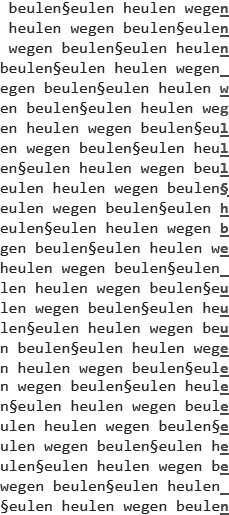
\includegraphics[height=0.725\textheight]{bwt/bwt_sort.png}
        %\includegraphics*[height=\textheight]{bwt/bwt_sort.png}
    \end{minipage}
\end{frame}

\begin{frame}
    \frametitle{Warum ist BWT sinnvoll?}
    \begin{columns}[T]
        \begin{column}{.33\textwidth}
            \centering
            \only<1-2>{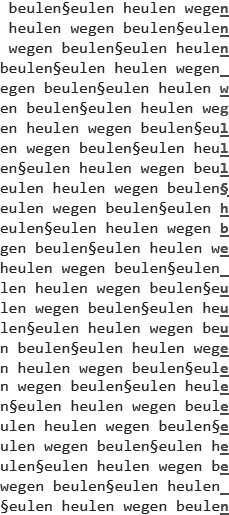
\includegraphics[height=0.725\textheight]{bwt/bwt_result.png}}
            \only<3-7>{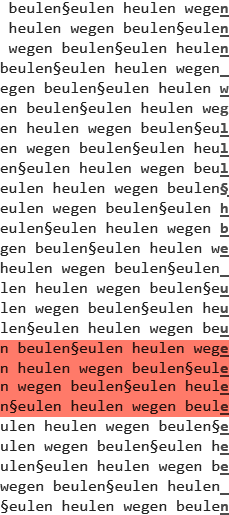
\includegraphics[height=0.725\textheight]{bwt/bwt_n.png}}
            \only<8>{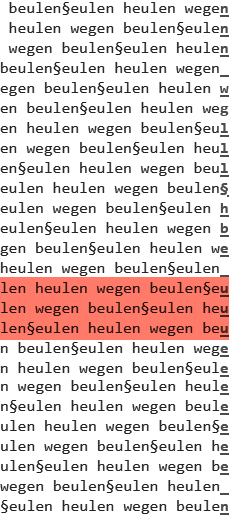
\includegraphics[height=0.725\textheight]{bwt/bwt_l.png}}
            \only<9>{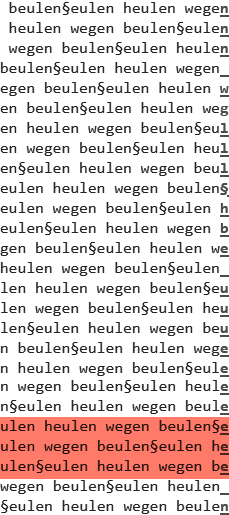
\includegraphics[height=0.725\textheight]{bwt/bwt_u.png}}
            \only<10->{
\includegraphics[height=0.725\textheight]{bwt/bwt_space.png}}
        \end{column}
        \hfill
        \begin{column}{.65\textwidth}
            \pause
            \begin{tcolorbox}[yellow]
                \begin{tabular}{rl}
                    \only<1-2,8->{Input: &eulen heulen wegen beulen\\
                    Output: &nnn wglll§hbe uuueeeeeee n}\noindent
                    \only<3-7>{Input: &eul\red{en} heul\red{en} weg\red{en} beul\red{en}\\
                    Output: &nnn wglll§hbe uuu\red{eeee}eee n}
                \end{tabular}
            \end{tcolorbox}\pause
            Betrachte die roten Zeilen:
            \begin{itemize}\pause
                \item \red{n} ist der erste Buchstabe der Zeilen\pause
                \begin{itemize}
                    \item Im Satz ist vor \red{n} immer ein \red{e}\pause
                \item Alle \red{e} sind in aufeinanderfolgenden Zeilen\pause
                \end{itemize}
                \item \"Ahnlich f\"ur \pause
                \red{u}\pause, \red{e}\pause~und \red{n}.
            \end{itemize}
            \vspace*{0.5cm}
        \end{column}
    \end{columns}
\end{frame}
\begin{frame}
    \frametitle{Warum ist der BWT sinnvoll?}
    \begin{tcolorbox}[yellow]
        \begin{center}
            \begin{tabular}{rl}
                Input: &eulen heulen wegen beulen\\
                Output: &nnn wglll§hbe uuueeeeeee n
            \end{tabular}
        \end{center}
    \end{tcolorbox}\pause\vspace*{0.3cm}
    Die Run-Length Enkodierung ergibt folgendes:\\~\\\pause
    \hspace*{0.3cm}
    Input \hspace*{0.3cm}$\overset{\text{RL}}{\R}$ 1e1u1l1e1n1 1h1e1u1l1e1n1 1w1e1g1e1n1 1b1e1u1l1e1n\\\pause
    \hspace*{0.3cm}
    Output $\overset{\text{RL}}{\R}$ 3n1 1w1g3l1§1h1b1e1 3u7e1 1n
    \pause\vspace*{0.3cm}
    \begin{tcolorbox}[standard, title=Wann ist BWT also sinnvoll:]
        \begin{itemize}
            \onslide<6->{\item Bei Texten mit vielen gleichen Buchstabenfolgen.}
            \onslide<7->{\item Gibt es in Sprachen sehr oft!}
        \end{itemize}
    \end{tcolorbox}
\end{frame}
\begin{frame}
    \frametitle{~}
    \begin{center}
        \Large{\blue{\textbf{Vielen Dank fürs Zuhören!}}}
    \end{center}
\end{frame}
\end{document}
